% Options for packages loaded elsewhere
\PassOptionsToPackage{unicode}{hyperref}
\PassOptionsToPackage{hyphens}{url}
%
\documentclass[
]{article}
\usepackage{amsmath,amssymb}
\usepackage{iftex}
\ifPDFTeX
  \usepackage[T1]{fontenc}
  \usepackage[utf8]{inputenc}
  \usepackage{textcomp} % provide euro and other symbols
\else % if luatex or xetex
  \usepackage{unicode-math} % this also loads fontspec
  \defaultfontfeatures{Scale=MatchLowercase}
  \defaultfontfeatures[\rmfamily]{Ligatures=TeX,Scale=1}
\fi
\usepackage{lmodern}
\ifPDFTeX\else
  % xetex/luatex font selection
\fi
% Use upquote if available, for straight quotes in verbatim environments
\IfFileExists{upquote.sty}{\usepackage{upquote}}{}
\IfFileExists{microtype.sty}{% use microtype if available
  \usepackage[]{microtype}
  \UseMicrotypeSet[protrusion]{basicmath} % disable protrusion for tt fonts
}{}
\makeatletter
\@ifundefined{KOMAClassName}{% if non-KOMA class
  \IfFileExists{parskip.sty}{%
    \usepackage{parskip}
  }{% else
    \setlength{\parindent}{0pt}
    \setlength{\parskip}{6pt plus 2pt minus 1pt}}
}{% if KOMA class
  \KOMAoptions{parskip=half}}
\makeatother
\usepackage{xcolor}
\usepackage[margin=1in]{geometry}
\usepackage{color}
\usepackage{fancyvrb}
\newcommand{\VerbBar}{|}
\newcommand{\VERB}{\Verb[commandchars=\\\{\}]}
\DefineVerbatimEnvironment{Highlighting}{Verbatim}{commandchars=\\\{\}}
% Add ',fontsize=\small' for more characters per line
\usepackage{framed}
\definecolor{shadecolor}{RGB}{248,248,248}
\newenvironment{Shaded}{\begin{snugshade}}{\end{snugshade}}
\newcommand{\AlertTok}[1]{\textcolor[rgb]{0.94,0.16,0.16}{#1}}
\newcommand{\AnnotationTok}[1]{\textcolor[rgb]{0.56,0.35,0.01}{\textbf{\textit{#1}}}}
\newcommand{\AttributeTok}[1]{\textcolor[rgb]{0.13,0.29,0.53}{#1}}
\newcommand{\BaseNTok}[1]{\textcolor[rgb]{0.00,0.00,0.81}{#1}}
\newcommand{\BuiltInTok}[1]{#1}
\newcommand{\CharTok}[1]{\textcolor[rgb]{0.31,0.60,0.02}{#1}}
\newcommand{\CommentTok}[1]{\textcolor[rgb]{0.56,0.35,0.01}{\textit{#1}}}
\newcommand{\CommentVarTok}[1]{\textcolor[rgb]{0.56,0.35,0.01}{\textbf{\textit{#1}}}}
\newcommand{\ConstantTok}[1]{\textcolor[rgb]{0.56,0.35,0.01}{#1}}
\newcommand{\ControlFlowTok}[1]{\textcolor[rgb]{0.13,0.29,0.53}{\textbf{#1}}}
\newcommand{\DataTypeTok}[1]{\textcolor[rgb]{0.13,0.29,0.53}{#1}}
\newcommand{\DecValTok}[1]{\textcolor[rgb]{0.00,0.00,0.81}{#1}}
\newcommand{\DocumentationTok}[1]{\textcolor[rgb]{0.56,0.35,0.01}{\textbf{\textit{#1}}}}
\newcommand{\ErrorTok}[1]{\textcolor[rgb]{0.64,0.00,0.00}{\textbf{#1}}}
\newcommand{\ExtensionTok}[1]{#1}
\newcommand{\FloatTok}[1]{\textcolor[rgb]{0.00,0.00,0.81}{#1}}
\newcommand{\FunctionTok}[1]{\textcolor[rgb]{0.13,0.29,0.53}{\textbf{#1}}}
\newcommand{\ImportTok}[1]{#1}
\newcommand{\InformationTok}[1]{\textcolor[rgb]{0.56,0.35,0.01}{\textbf{\textit{#1}}}}
\newcommand{\KeywordTok}[1]{\textcolor[rgb]{0.13,0.29,0.53}{\textbf{#1}}}
\newcommand{\NormalTok}[1]{#1}
\newcommand{\OperatorTok}[1]{\textcolor[rgb]{0.81,0.36,0.00}{\textbf{#1}}}
\newcommand{\OtherTok}[1]{\textcolor[rgb]{0.56,0.35,0.01}{#1}}
\newcommand{\PreprocessorTok}[1]{\textcolor[rgb]{0.56,0.35,0.01}{\textit{#1}}}
\newcommand{\RegionMarkerTok}[1]{#1}
\newcommand{\SpecialCharTok}[1]{\textcolor[rgb]{0.81,0.36,0.00}{\textbf{#1}}}
\newcommand{\SpecialStringTok}[1]{\textcolor[rgb]{0.31,0.60,0.02}{#1}}
\newcommand{\StringTok}[1]{\textcolor[rgb]{0.31,0.60,0.02}{#1}}
\newcommand{\VariableTok}[1]{\textcolor[rgb]{0.00,0.00,0.00}{#1}}
\newcommand{\VerbatimStringTok}[1]{\textcolor[rgb]{0.31,0.60,0.02}{#1}}
\newcommand{\WarningTok}[1]{\textcolor[rgb]{0.56,0.35,0.01}{\textbf{\textit{#1}}}}
\usepackage{graphicx}
\makeatletter
\def\maxwidth{\ifdim\Gin@nat@width>\linewidth\linewidth\else\Gin@nat@width\fi}
\def\maxheight{\ifdim\Gin@nat@height>\textheight\textheight\else\Gin@nat@height\fi}
\makeatother
% Scale images if necessary, so that they will not overflow the page
% margins by default, and it is still possible to overwrite the defaults
% using explicit options in \includegraphics[width, height, ...]{}
\setkeys{Gin}{width=\maxwidth,height=\maxheight,keepaspectratio}
% Set default figure placement to htbp
\makeatletter
\def\fps@figure{htbp}
\makeatother
\setlength{\emergencystretch}{3em} % prevent overfull lines
\providecommand{\tightlist}{%
  \setlength{\itemsep}{0pt}\setlength{\parskip}{0pt}}
\setcounter{secnumdepth}{-\maxdimen} % remove section numbering
\ifLuaTeX
  \usepackage{selnolig}  % disable illegal ligatures
\fi
\usepackage{bookmark}
\IfFileExists{xurl.sty}{\usepackage{xurl}}{} % add URL line breaks if available
\urlstyle{same}
\hypersetup{
  pdftitle={PEC 1: Informe de Análisis Metabolómico de orina en mujeres después de beber zumo de arándano o manzana},
  pdfauthor={Gabriel Manzano Reche},
  hidelinks,
  pdfcreator={LaTeX via pandoc}}

\title{PEC 1: Informe de Análisis Metabolómico de orina en mujeres
después de beber zumo de arándano o manzana}
\author{Gabriel Manzano Reche}
\date{\emph{28 de octubre de 2024}}

\begin{document}
\maketitle

{
\setcounter{tocdepth}{2}
\tableofcontents
}
\pagebreak

\section{1. Introducción}\label{introducciuxf3n}

Para esta PEC1 se ha escogido el dataset propuesto llamado
\textbf{2018-Phosphoproteomics}.

Los daros de este estudio se han obtenido a partir de un experimento de
fosfoproteómica. El experimento ha analizado (3 + 3) modelos PDX de dos
subtipos diferentes utilizando muestras enriquecidas en fosfopéptidos.
Se realizó un análisis LC-MS con 2 réplicas técnicas para cada muestra.
El conjunto de resultados consiste en abundancias normalizadas de
señales MS para aproximadamente 1400 fosfopéptidos. El objetivo del
análisis es identificar fosfopéptidos que permitan diferenciar los dos
grupos de tumores. Esto debe realizarse mediante análisis estadístico y
visualización. Los datos se han proporcionado en un archivo de Excel:
TIO2+PTYR-human-MSS+MSIvsPD.XLSX.

Los grupos están definidos como:

\begin{itemize}
\tightlist
\item
  Grupo MSS: Muestras M1, M5 y T49
\item
  Grupo PD: Muestras M42, M43 y M64
\end{itemize}

Cada muestra cuenta con dos réplicas técnicas. La primera columna,
SequenceModification, contiene los valores de abundancia para los
distintos fosfopéptidos. Las demás columnas pueden omitirse.

\section{2. Carga de los datos}\label{carga-de-los-datos}

\begin{Shaded}
\begin{Highlighting}[]
\FunctionTok{library}\NormalTok{(SummarizedExperiment)}
\end{Highlighting}
\end{Shaded}

\begin{verbatim}
## Loading required package: MatrixGenerics
\end{verbatim}

\begin{verbatim}
## Loading required package: matrixStats
\end{verbatim}

\begin{verbatim}
## 
## Attaching package: 'MatrixGenerics'
\end{verbatim}

\begin{verbatim}
## The following objects are masked from 'package:matrixStats':
## 
##     colAlls, colAnyNAs, colAnys, colAvgsPerRowSet, colCollapse,
##     colCounts, colCummaxs, colCummins, colCumprods, colCumsums,
##     colDiffs, colIQRDiffs, colIQRs, colLogSumExps, colMadDiffs,
##     colMads, colMaxs, colMeans2, colMedians, colMins, colOrderStats,
##     colProds, colQuantiles, colRanges, colRanks, colSdDiffs, colSds,
##     colSums2, colTabulates, colVarDiffs, colVars, colWeightedMads,
##     colWeightedMeans, colWeightedMedians, colWeightedSds,
##     colWeightedVars, rowAlls, rowAnyNAs, rowAnys, rowAvgsPerColSet,
##     rowCollapse, rowCounts, rowCummaxs, rowCummins, rowCumprods,
##     rowCumsums, rowDiffs, rowIQRDiffs, rowIQRs, rowLogSumExps,
##     rowMadDiffs, rowMads, rowMaxs, rowMeans2, rowMedians, rowMins,
##     rowOrderStats, rowProds, rowQuantiles, rowRanges, rowRanks,
##     rowSdDiffs, rowSds, rowSums2, rowTabulates, rowVarDiffs, rowVars,
##     rowWeightedMads, rowWeightedMeans, rowWeightedMedians,
##     rowWeightedSds, rowWeightedVars
\end{verbatim}

\begin{verbatim}
## Loading required package: GenomicRanges
\end{verbatim}

\begin{verbatim}
## Loading required package: stats4
\end{verbatim}

\begin{verbatim}
## Loading required package: BiocGenerics
\end{verbatim}

\begin{verbatim}
## 
## Attaching package: 'BiocGenerics'
\end{verbatim}

\begin{verbatim}
## The following objects are masked from 'package:stats':
## 
##     IQR, mad, sd, var, xtabs
\end{verbatim}

\begin{verbatim}
## The following objects are masked from 'package:base':
## 
##     anyDuplicated, aperm, append, as.data.frame, basename, cbind,
##     colnames, dirname, do.call, duplicated, eval, evalq, Filter, Find,
##     get, grep, grepl, intersect, is.unsorted, lapply, Map, mapply,
##     match, mget, order, paste, pmax, pmax.int, pmin, pmin.int,
##     Position, rank, rbind, Reduce, rownames, sapply, setdiff, sort,
##     table, tapply, union, unique, unsplit, which.max, which.min
\end{verbatim}

\begin{verbatim}
## Loading required package: S4Vectors
\end{verbatim}

\begin{verbatim}
## 
## Attaching package: 'S4Vectors'
\end{verbatim}

\begin{verbatim}
## The following object is masked from 'package:utils':
## 
##     findMatches
\end{verbatim}

\begin{verbatim}
## The following objects are masked from 'package:base':
## 
##     expand.grid, I, unname
\end{verbatim}

\begin{verbatim}
## Loading required package: IRanges
\end{verbatim}

\begin{verbatim}
## 
## Attaching package: 'IRanges'
\end{verbatim}

\begin{verbatim}
## The following object is masked from 'package:grDevices':
## 
##     windows
\end{verbatim}

\begin{verbatim}
## Loading required package: GenomeInfoDb
\end{verbatim}

\begin{verbatim}
## Loading required package: Biobase
\end{verbatim}

\begin{verbatim}
## Welcome to Bioconductor
## 
##     Vignettes contain introductory material; view with
##     'browseVignettes()'. To cite Bioconductor, see
##     'citation("Biobase")', and for packages 'citation("pkgname")'.
\end{verbatim}

\begin{verbatim}
## 
## Attaching package: 'Biobase'
\end{verbatim}

\begin{verbatim}
## The following object is masked from 'package:MatrixGenerics':
## 
##     rowMedians
\end{verbatim}

\begin{verbatim}
## The following objects are masked from 'package:matrixStats':
## 
##     anyMissing, rowMedians
\end{verbatim}

\begin{Shaded}
\begin{Highlighting}[]
\FunctionTok{library}\NormalTok{(readxl)}
\FunctionTok{library}\NormalTok{(tidyverse)}
\end{Highlighting}
\end{Shaded}

\begin{verbatim}
## -- Attaching core tidyverse packages ------------------------ tidyverse 2.0.0 --
## v dplyr     1.1.4     v readr     2.1.5
## v forcats   1.0.0     v stringr   1.5.1
## v ggplot2   3.5.1     v tibble    3.2.1
## v lubridate 1.9.3     v tidyr     1.3.1
## v purrr     1.0.2
\end{verbatim}

\begin{verbatim}
## -- Conflicts ------------------------------------------ tidyverse_conflicts() --
## x lubridate::%within%() masks IRanges::%within%()
## x dplyr::collapse()     masks IRanges::collapse()
## x dplyr::combine()      masks Biobase::combine(), BiocGenerics::combine()
## x dplyr::count()        masks matrixStats::count()
## x dplyr::desc()         masks IRanges::desc()
## x tidyr::expand()       masks S4Vectors::expand()
## x dplyr::filter()       masks stats::filter()
## x dplyr::first()        masks S4Vectors::first()
## x dplyr::lag()          masks stats::lag()
## x ggplot2::Position()   masks BiocGenerics::Position(), base::Position()
## x purrr::reduce()       masks GenomicRanges::reduce(), IRanges::reduce()
## x dplyr::rename()       masks S4Vectors::rename()
## x lubridate::second()   masks S4Vectors::second()
## x lubridate::second<-() masks S4Vectors::second<-()
## x dplyr::slice()        masks IRanges::slice()
## i Use the conflicted package (<http://conflicted.r-lib.org/>) to force all conflicts to become errors
\end{verbatim}

\begin{Shaded}
\begin{Highlighting}[]
\CommentTok{\# Carga de los datos de la hoja 1}
\NormalTok{original\_data }\OtherTok{\textless{}{-}} \FunctionTok{read\_excel}\NormalTok{(}\StringTok{"TIO2+PTYR{-}human{-}MSS+MSIvsPD.XLSX"}\NormalTok{)}
\FunctionTok{head}\NormalTok{(original\_data)}
\end{Highlighting}
\end{Shaded}

\begin{verbatim}
## # A tibble: 6 x 18
##   SequenceModifications   Accession Description Score M1_1_MSS M1_2_MSS M5_1_MSS
##   <chr>                   <chr>     <chr>       <dbl>    <dbl>    <dbl>    <dbl>
## 1 LYPELSQYMGLSLNEEEIR[2]~ O00560    Syntenin-1~  48.1     24.3   44476.       0 
## 2 VDKVIQAQTAFSANPANPAILS~ O00560    Syntenin-1~  67.0      0     43139.    2102.
## 3 VIQAQTAFSANPANPAILSEAS~ O00560    Syntenin-1~  77.7   3413.   172143.   77323.
## 4 HADAEMTGYVVTR[6] Oxida~ O15264    Mitogen-ac~  44.9 220431.   145657.  104288.
## 5 HADAEMTGYVVTR[9] Phosp~ O15264    Mitogen-ac~  67.4  18255.     8530.   35956.
## 6 STGPGASLGTGYDR[12] Pho~ O15551    Claudin-3 ~  63.7 644513.   261938.  187023.
## # i 11 more variables: M5_2_MSS <dbl>, T49_1_MSS <dbl>, T49_2_MSS <dbl>,
## #   M42_1_PD <dbl>, M42_2_PD <dbl>, M43_1_PD <dbl>, M43_2_PD <dbl>,
## #   M64_1_PD <dbl>, M64_2_PD <dbl>, CLASS <chr>, PHOSPHO <chr>
\end{verbatim}

\begin{Shaded}
\begin{Highlighting}[]
\CommentTok{\# Carga de los datos de la hoja 1}
\NormalTok{targets }\OtherTok{\textless{}{-}} \FunctionTok{read\_excel}\NormalTok{(}\StringTok{"TIO2+PTYR{-}human{-}MSS+MSIvsPD.XLSX"}\NormalTok{, }\AttributeTok{sheet =} \DecValTok{2}\NormalTok{)}
\end{Highlighting}
\end{Shaded}

\begin{verbatim}
## New names:
## * `Sample` -> `Sample...1`
## * `Sample` -> `Sample...2`
\end{verbatim}

\begin{Shaded}
\begin{Highlighting}[]
\FunctionTok{head}\NormalTok{(targets)}
\end{Highlighting}
\end{Shaded}

\begin{verbatim}
## # A tibble: 6 x 4
##   Sample...1 Sample...2 Individual Phenotype
##   <chr>      <chr>           <dbl> <chr>    
## 1 M1_1       M1                  1 MSS      
## 2 M1_2       M1                  1 MSS      
## 3 M5_1       M5                  2 MSS      
## 4 M5_2       M5                  2 MSS      
## 5 T49_1      T49                 3 MSS      
## 6 T49_2      T49                 3 MSS
\end{verbatim}

\begin{Shaded}
\begin{Highlighting}[]
\CommentTok{\# Nombres de las columnas}
\FunctionTok{colnames}\NormalTok{(original\_data)}
\end{Highlighting}
\end{Shaded}

\begin{verbatim}
##  [1] "SequenceModifications" "Accession"             "Description"          
##  [4] "Score"                 "M1_1_MSS"              "M1_2_MSS"             
##  [7] "M5_1_MSS"              "M5_2_MSS"              "T49_1_MSS"            
## [10] "T49_2_MSS"             "M42_1_PD"              "M42_2_PD"             
## [13] "M43_1_PD"              "M43_2_PD"              "M64_1_PD"             
## [16] "M64_2_PD"              "CLASS"                 "PHOSPHO"
\end{verbatim}

Como se puede ver de la columna 5 a la 16, se encuentran las
abundancias. Estás se almacenarán en un nuevo dataframe llamado
abundancias y se le asignarán el nombre de los fosfopéptidos a las
filas, los cuales se encuentran en la columna Accesion.

\section{3. Seleccionar columna de metadatos y
datos}\label{seleccionar-columna-de-metadatos-y-datos}

\begin{Shaded}
\begin{Highlighting}[]
\CommentTok{\# Seleccionar las columnas de abundancia y almacenarlas en una variable}
\NormalTok{abundancias }\OtherTok{\textless{}{-}}\NormalTok{ original\_data }\SpecialCharTok{\%\textgreater{}\%} \FunctionTok{select}\NormalTok{(}\DecValTok{5}\SpecialCharTok{:}\DecValTok{16}\NormalTok{)}
\NormalTok{abundancias }\OtherTok{\textless{}{-}} \FunctionTok{as.data.frame}\NormalTok{(abundancias)}

\CommentTok{\# Asignarle nuevos nombres a las columnas de la matriz de abundancia}
\NormalTok{accesion\_rownames }\OtherTok{\textless{}{-}} \FunctionTok{make.names}\NormalTok{(original\_data}\SpecialCharTok{$}\NormalTok{Accession, }\AttributeTok{unique =} \ConstantTok{TRUE}\NormalTok{)}
\FunctionTok{rownames}\NormalTok{(abundancias) }\OtherTok{\textless{}{-}}\NormalTok{ accesion\_rownames}
\FunctionTok{head}\NormalTok{(abundancias)}
\end{Highlighting}
\end{Shaded}

\begin{verbatim}
##              M1_1_MSS   M1_2_MSS   M5_1_MSS   M5_2_MSS    T49_1_MSS  T49_2_MSS
## O00560       24.29438  44475.964      0.000   6269.141    1135.8169   21933.90
## O00560.1      0.00000  43138.904   2102.056  50355.051     248.9275    3239.16
## O00560.2   3412.60332 172143.040  77323.019 307637.429   98442.2773  192982.37
## O15264   220431.17880 145656.887 104287.815  75887.365  773377.4981  481165.54
## O15264.1  18254.77813   8529.755  35955.901  44102.316   57145.1682   34638.01
## O15551   644513.31840 261938.025 187023.484 124867.715 4487443.6920 2572575.27
##             M42_1_PD   M42_2_PD     M43_1_PD    M43_2_PD    M64_1_PD
## O00560         0.000       0.00     772.9056    2136.746    1820.724
## O00560.1    1315.904       0.00       0.0000       0.000       0.000
## O00560.2   24851.344   16547.95    5565.2821       0.000    3264.563
## O15264   1027196.292 1163747.38 4080239.1820 4885818.113 3093786.793
## O15264.1   21231.256   49499.70  666107.0448  379313.615  255792.117
## O15551    535809.187  434645.89   91361.8781   65997.913  243250.439
##              M64_2_PD
## O00560      1727.9098
## O00560.1     892.3565
## O00560.2    5901.9577
## O15264   2759104.5440
## O15264.1  579765.0018
## O15551    206632.6444
\end{verbatim}

A continuación se definen los metadatos, que incluyen información de las
muestras como grupo y réplica, y detalles de los fosfopéptidos como
modificaciones de secuencia y descripción.

En primer lugar, se definen los metadatos de las muestras que se
almacenarán en la variable sample\_info. Esta variable contiene el
SampleID de cada muestra, el grupo y el número de réplica.

\begin{Shaded}
\begin{Highlighting}[]
\CommentTok{\# Crear el DataFrame de metadatos de las muestras}
\NormalTok{sample\_info }\OtherTok{\textless{}{-}} \FunctionTok{DataFrame}\NormalTok{(}
    \AttributeTok{SampleID =} \FunctionTok{colnames}\NormalTok{(abundancias),}
    \AttributeTok{Group =} \FunctionTok{c}\NormalTok{(}\FunctionTok{rep}\NormalTok{(}\StringTok{"MSS"}\NormalTok{, }\DecValTok{6}\NormalTok{), }\FunctionTok{rep}\NormalTok{(}\StringTok{"PD"}\NormalTok{, }\DecValTok{6}\NormalTok{)),}
    \AttributeTok{Replicate =} \FunctionTok{rep}\NormalTok{(}\FunctionTok{c}\NormalTok{(}\DecValTok{1}\NormalTok{, }\DecValTok{2}\NormalTok{), }\AttributeTok{times =} \DecValTok{6}\NormalTok{)}
\NormalTok{)}
\end{Highlighting}
\end{Shaded}

A continuación se definen los metadatos de los fosfopéptidos, una
descripción de estos y la modificacion en su secuencia.

\begin{Shaded}
\begin{Highlighting}[]
\CommentTok{\# Crear el DataFrame con metadatos de los fosfopéptidos}
\NormalTok{row\_data }\OtherTok{\textless{}{-}} \FunctionTok{DataFrame}\NormalTok{(}
    \AttributeTok{SequenceModifications =}\NormalTok{ original\_data}\SpecialCharTok{$}\NormalTok{SequenceModifications,}
    \AttributeTok{Description =}\NormalTok{ original\_data}\SpecialCharTok{$}\NormalTok{Description,}
    \AttributeTok{row.names =} \FunctionTok{rownames}\NormalTok{(abundancias)}
\NormalTok{)}
\end{Highlighting}
\end{Shaded}

\section{\texorpdfstring{3. Crear y explorar el objeto
\emph{SummarizedData}}{3. Crear y explorar el objeto SummarizedData}}\label{crear-y-explorar-el-objeto-summarizeddata}

Finalmente, se crea el objeto \emph{SummarizedData} que permite
organizar la matriz de abundancia junto con los metadatos en un solo
objeto, facilitando el análisis de los datos.

\begin{Shaded}
\begin{Highlighting}[]
\CommentTok{\# Crear el objeto SummarizedExperiment}
\NormalTok{se }\OtherTok{\textless{}{-}} \FunctionTok{SummarizedExperiment}\NormalTok{(}
    \AttributeTok{assays =} \FunctionTok{list}\NormalTok{(}\AttributeTok{counts =} \FunctionTok{as.matrix}\NormalTok{(abundancias)),  }\CommentTok{\# Matriz de abundancia}
    \AttributeTok{colData =}\NormalTok{ sample\_info,  }\CommentTok{\# Metadata de las muestras}
    \AttributeTok{rowData =}\NormalTok{ row\_data  }\CommentTok{\# Metadata de los fosfopéptidos}
\NormalTok{)}

\NormalTok{se}
\end{Highlighting}
\end{Shaded}

\begin{verbatim}
## class: SummarizedExperiment 
## dim: 1438 12 
## metadata(0):
## assays(1): counts
## rownames(1438): O00560 O00560.1 ... Q13283.1 Q9NYF8.12
## rowData names(2): SequenceModifications Description
## colnames(12): M1_1_MSS M1_2_MSS ... M64_1_PD M64_2_PD
## colData names(3): SampleID Group Replicate
\end{verbatim}

\section{4. Análisis de los datos}\label{anuxe1lisis-de-los-datos}

\begin{Shaded}
\begin{Highlighting}[]
\CommentTok{\# Resumen estadístico de la matriz de abundancia}
\FunctionTok{summary}\NormalTok{(}\FunctionTok{assay}\NormalTok{(se, }\StringTok{"counts"}\NormalTok{))}
\end{Highlighting}
\end{Shaded}

\begin{verbatim}
##     M1_1_MSS           M1_2_MSS           M5_1_MSS           M5_2_MSS       
##  Min.   :       0   Min.   :       0   Min.   :       0   Min.   :       0  
##  1st Qu.:    5653   1st Qu.:    5497   1st Qu.:    2573   1st Qu.:    3273  
##  Median :   30682   Median :   26980   Median :   20801   Median :   26241  
##  Mean   :  229841   Mean   :  253151   Mean   :  232967   Mean   :  261067  
##  3rd Qu.:  117373   3rd Qu.:  113004   3rd Qu.:  113958   3rd Qu.:  130132  
##  Max.   :16719906   Max.   :43928481   Max.   :15135169   Max.   :19631820  
##    T49_1_MSS          T49_2_MSS           M42_1_PD           M42_2_PD       
##  Min.   :       0   Min.   :       0   Min.   :       0   Min.   :       0  
##  1st Qu.:    9306   1st Qu.:    8611   1st Qu.:    5341   1st Qu.:    4216  
##  Median :   55641   Median :   46110   Median :   36854   Median :   30533  
##  Mean   :  542449   Mean   :  462616   Mean   :  388424   Mean   :  333587  
##  3rd Qu.:  223103   3rd Qu.:  189141   3rd Qu.:  180252   3rd Qu.:  152088  
##  Max.   :49218872   Max.   :29240206   Max.   :48177680   Max.   :42558111  
##     M43_1_PD           M43_2_PD           M64_1_PD           M64_2_PD       
##  Min.   :       0   Min.   :       0   Min.   :       0   Min.   :       0  
##  1st Qu.:   19641   1st Qu.:   17299   1st Qu.:   11038   1st Qu.:    8660  
##  Median :   67945   Median :   59607   Median :   52249   Median :   47330  
##  Mean   :  349020   Mean   :  358822   Mean   :  470655   Mean   :  484712  
##  3rd Qu.:  205471   3rd Qu.:  201924   3rd Qu.:  209896   3rd Qu.:  206036  
##  Max.   :35049402   Max.   :63082982   Max.   :71750330   Max.   :88912734
\end{verbatim}

\begin{Shaded}
\begin{Highlighting}[]
\CommentTok{\# Convertir los datos de abundancia a formato largo}
\NormalTok{abundances\_long }\OtherTok{\textless{}{-}}\NormalTok{ abundancias }\SpecialCharTok{\%\textgreater{}\%} 
  \FunctionTok{pivot\_longer}\NormalTok{(}\AttributeTok{cols =} \FunctionTok{everything}\NormalTok{(), }\AttributeTok{names\_to =} \StringTok{"Muestra"}\NormalTok{, }\AttributeTok{values\_to =} \StringTok{"Abundancia"}\NormalTok{)}

\CommentTok{\# Crear el histograma para cada muestra}
\FunctionTok{ggplot}\NormalTok{(abundances\_long, }\FunctionTok{aes}\NormalTok{(}\AttributeTok{x =}\NormalTok{ Abundancia)) }\SpecialCharTok{+}
  \FunctionTok{geom\_histogram}\NormalTok{(}\AttributeTok{bins =} \DecValTok{20}\NormalTok{, }\AttributeTok{fill =} \StringTok{"red"}\NormalTok{, }\AttributeTok{color =} \StringTok{"black"}\NormalTok{) }\SpecialCharTok{+}
  \FunctionTok{facet\_wrap}\NormalTok{(}\SpecialCharTok{\textasciitilde{}}\NormalTok{ Muestra, }\AttributeTok{scales =} \StringTok{"free\_x"}\NormalTok{) }\SpecialCharTok{+}  \CommentTok{\# Crear un gráfico por cada muestra}
  \FunctionTok{labs}\NormalTok{(}\AttributeTok{title =} \StringTok{"Distribución de abundancias en cada muestra"}\NormalTok{,}
       \AttributeTok{x =} \StringTok{"Abundancia"}\NormalTok{,}
       \AttributeTok{y =} \StringTok{"Frecuencia"}\NormalTok{) }\SpecialCharTok{+}
  \FunctionTok{theme\_minimal}\NormalTok{()}
\end{Highlighting}
\end{Shaded}

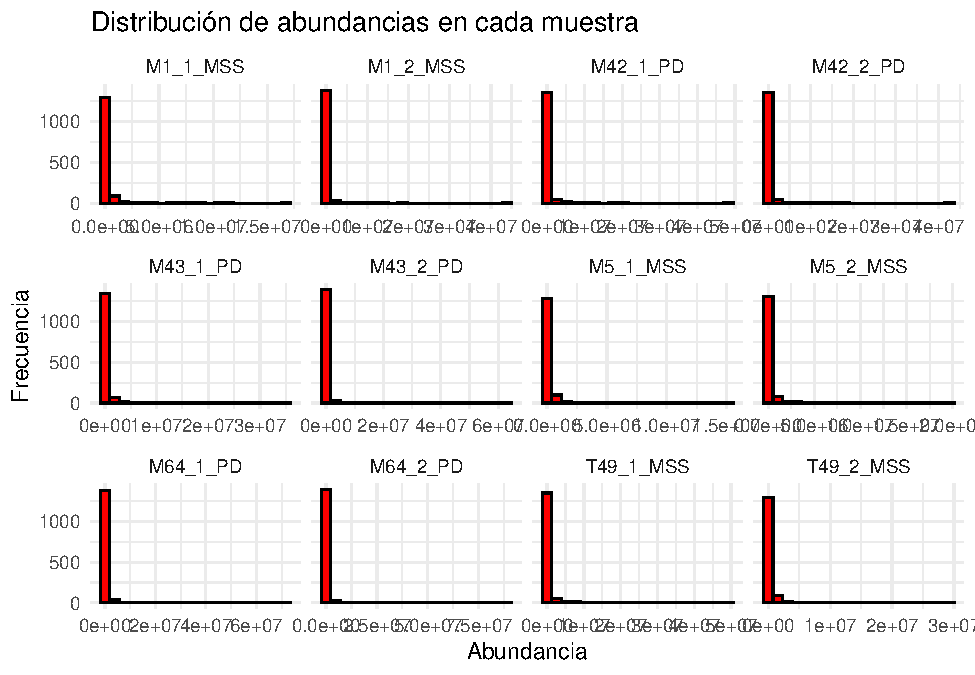
\includegraphics{Manzano-Reche-Gabriel-PEC1_files/figure-latex/unnamed-chunk-10-1.pdf}

Como se puede apreciar en los histogramas de arriba, todas las muestras
están sesgadas hacia la izquierda. Esto sugiere que puede ser útil
normalizar los datos (aplicando log10) para visualizar mejor las
diferencias entre las muestras. A continuación se viualizarán las datos
normalizados en base 10

\begin{Shaded}
\begin{Highlighting}[]
\CommentTok{\# Visualizar distribuciones de abundancia en escala logarítmica}
\FunctionTok{boxplot}\NormalTok{(}\FunctionTok{log10}\NormalTok{(}\FunctionTok{assay}\NormalTok{(se, }\StringTok{"counts"}\NormalTok{) }\SpecialCharTok{+} \DecValTok{1}\NormalTok{), }
        \AttributeTok{main =} \StringTok{"Distribución de abundancias en escala log10"}\NormalTok{,}
        \AttributeTok{xlab =} \StringTok{"Muestras"}\NormalTok{,}
        \AttributeTok{ylab =} \StringTok{"Log10(Abundancia + 1)"}\NormalTok{,}
        \AttributeTok{las =} \DecValTok{2}\NormalTok{,  }\CommentTok{\# Gira las etiquetas del eje x para facilitar la lectura}
        \AttributeTok{col =} \StringTok{"lightblue"}\NormalTok{,  }\CommentTok{\# Color de las cajas}
        \AttributeTok{border =} \StringTok{"darkblue"}\NormalTok{)  }\CommentTok{\# Color del borde}
\end{Highlighting}
\end{Shaded}

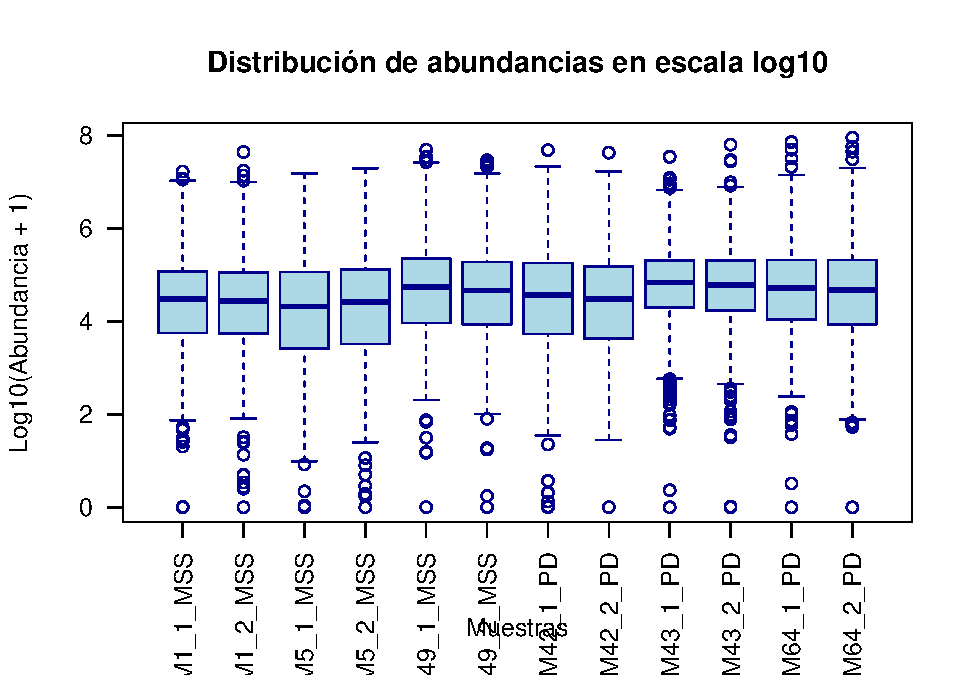
\includegraphics{Manzano-Reche-Gabriel-PEC1_files/figure-latex/unnamed-chunk-11-1.pdf}

En este gráfico se puede observar la distribución de las abundacias de
péptidos en las muestras en escala logarítmica, en donde no se observa
una separación clara entre las muestras de los grupos MSS y PD.

A continuación, se normalizarán los datos de la matriz de abundancias y
se extraerá el grupo y réplica a la que pertenece cada muestra, con el
objetivo de identificar diferencias significativas entre grupos o entre
réplicas.

\begin{Shaded}
\begin{Highlighting}[]
\CommentTok{\# Extraer la matriz de abundancia del objeto SummarizedExperiment}
\NormalTok{abundancias }\OtherTok{\textless{}{-}} \FunctionTok{assay}\NormalTok{(se, }\StringTok{"counts"}\NormalTok{)}

\CommentTok{\# Convertir la matriz de abundancia a formato largo y aplicar transformación logarítmica}
\NormalTok{logDat }\OtherTok{\textless{}{-}} \FunctionTok{as.data.frame}\NormalTok{(abundancias) }\SpecialCharTok{\%\textgreater{}\%}
  \FunctionTok{pivot\_longer}\NormalTok{(}\AttributeTok{cols =} \FunctionTok{everything}\NormalTok{(), }\AttributeTok{names\_to =} \StringTok{"Muestra"}\NormalTok{, }\AttributeTok{values\_to =} \StringTok{"Abundancia"}\NormalTok{) }\SpecialCharTok{\%\textgreater{}\%}
  \FunctionTok{mutate}\NormalTok{(}\AttributeTok{logvalues =} \FunctionTok{log10}\NormalTok{(Abundancia }\SpecialCharTok{+} \DecValTok{1}\NormalTok{))}

\CommentTok{\# Extraer información de Grupo y Réplica desde el nombre de la muestra}
\NormalTok{covs }\OtherTok{\textless{}{-}} \FunctionTok{str\_split}\NormalTok{(logDat}\SpecialCharTok{$}\NormalTok{Muestra, }\StringTok{"\_"}\NormalTok{, }\AttributeTok{simplify =} \ConstantTok{TRUE}\NormalTok{)}
\FunctionTok{colnames}\NormalTok{(covs) }\OtherTok{\textless{}{-}} \FunctionTok{c}\NormalTok{(}\StringTok{"Sample"}\NormalTok{, }\StringTok{"Replicate"}\NormalTok{, }\StringTok{"Group"}\NormalTok{)}

\CommentTok{\# Añadir las nuevas columnas (Sample, Replicate, Group) al dataframe logDat}
\NormalTok{logDat2 }\OtherTok{\textless{}{-}} \FunctionTok{cbind}\NormalTok{(logDat, covs)}

\CommentTok{\# Verificar la estructura de los datos transformados}
\FunctionTok{head}\NormalTok{(logDat2)}
\end{Highlighting}
\end{Shaded}

\begin{verbatim}
##     Muestra  Abundancia logvalues Sample Replicate Group
## 1  M1_1_MSS    24.29438  1.403024     M1         1   MSS
## 2  M1_2_MSS 44475.96381  4.648135     M1         2   MSS
## 3  M5_1_MSS     0.00000  0.000000     M5         1   MSS
## 4  M5_2_MSS  6269.14095  3.797277     M5         2   MSS
## 5 T49_1_MSS  1135.81687  3.055691    T49         1   MSS
## 6 T49_2_MSS 21933.89963  4.341136    T49         2   MSS
\end{verbatim}

\begin{Shaded}
\begin{Highlighting}[]
\CommentTok{\# Crear el boxplot con ggplot2 usando el grupo y la réplica como variables estéticas}
\FunctionTok{ggplot}\NormalTok{(logDat2, }\FunctionTok{aes}\NormalTok{(}\AttributeTok{x =}\NormalTok{ Muestra, }\AttributeTok{y =}\NormalTok{ logvalues, }\AttributeTok{fill =}\NormalTok{ Group, }\AttributeTok{colour =}\NormalTok{ Replicate)) }\SpecialCharTok{+} 
  \FunctionTok{geom\_boxplot}\NormalTok{() }\SpecialCharTok{+}
  \FunctionTok{theme}\NormalTok{(}\AttributeTok{axis.text.x =} \FunctionTok{element\_text}\NormalTok{(}\AttributeTok{angle =} \DecValTok{90}\NormalTok{, }\AttributeTok{hjust =} \DecValTok{1}\NormalTok{)) }\SpecialCharTok{+}
  \FunctionTok{labs}\NormalTok{(}\AttributeTok{title =} \StringTok{"Distribución de abundancias de fosfopéptidos (escala log10)"}\NormalTok{,}
       \AttributeTok{x =} \StringTok{"Muestras"}\NormalTok{,}
       \AttributeTok{y =} \StringTok{"Log10(Abundancia + 1)"}\NormalTok{)}
\end{Highlighting}
\end{Shaded}

\includegraphics{Manzano-Reche-Gabriel-PEC1_files/figure-latex/unnamed-chunk-13-1.pdf}

Este gráfico muestra la distribución de abundacias de fosfopéptidos en
escala logarítmo para cada muestra, representando también el grupo y la
réplica a la que pertenece esa muestra. No se aprecia diferencia
significativa entre los grupos ni entre las réplicas.

\subsection{Análisis de Componentes
Principales}\label{anuxe1lisis-de-componentes-principales}

\begin{Shaded}
\begin{Highlighting}[]
\CommentTok{\# Análisis de Componentes Principales}
\FunctionTok{source}\NormalTok{(}\StringTok{"https://raw.githubusercontent.com/uebvhir/UEB\_PCA/master/UEB\_plotPCA3.R"}\NormalTok{)}
\end{Highlighting}
\end{Shaded}

\begin{verbatim}
## Loading required package: ggrepel
\end{verbatim}

\begin{Shaded}
\begin{Highlighting}[]
\FunctionTok{plotPCA3}\NormalTok{(}\AttributeTok{datos=}\FunctionTok{as.matrix}\NormalTok{(}\FunctionTok{log10}\NormalTok{(abundancias}\SpecialCharTok{+}\DecValTok{1}\NormalTok{)), }\AttributeTok{labels=}\FunctionTok{colnames}\NormalTok{(abundancias), }
         \AttributeTok{factor=}\NormalTok{targets}\SpecialCharTok{$}\NormalTok{Phenotype, }\AttributeTok{title =}\StringTok{"Phosphoproteomic data"}\NormalTok{,}
         \AttributeTok{scale=}\ConstantTok{FALSE}\NormalTok{, }\AttributeTok{colores=}\DecValTok{1}\SpecialCharTok{:}\DecValTok{2}\NormalTok{, }\AttributeTok{size =} \FloatTok{3.5}\NormalTok{, }\AttributeTok{glineas =} \FloatTok{2.5}\NormalTok{)}
\end{Highlighting}
\end{Shaded}

\includegraphics{Manzano-Reche-Gabriel-PEC1_files/figure-latex/unnamed-chunk-14-1.pdf}

Este gráfico muestra el resultado de aplicar el análisis de componentes
principales sobre los datos. En el eje X se representa la componente
principal 1 y en el eje y la componente principal 2.

Se puede apreciar una clara separación entre los grupos MSS y PD, lo que
indica que estos dos grupos presentan diferencias significativas, las
cuales no se habían podido apreciar en los análisis anteriores. Además,
también se puede ver que mientras las muestras el grupo MSS permanecen
agrupadas, las muestras del grupo PD están muy dispersas, lo que indica
heterogeneidad en el grupo.

\section{Repositorio de Github}\label{repositorio-de-github}

A continuación se muestra los comandos utilizados para crear el
repositorio Github:

\begin{itemize}
\tightlist
\item
  En primer lugar, se crea el repositorio en mi cuenta de Github y lo
  llamamos Manzano-Reche-Gabriel-PEC1
\end{itemize}

\begin{Shaded}
\begin{Highlighting}[]
\CommentTok{\# Iniciar Git en local}
\NormalTok{git init}

\CommentTok{\# Añadir archivos presentes en el path}
\FunctionTok{system}\NormalTok{(}\StringTok{"git add ."}\NormalTok{)}

\CommentTok{\# Realizar un commmit}
\FunctionTok{system}\NormalTok{(}\StringTok{\textquotesingle{}git command {-}m "Mensaje"\textquotesingle{}}\NormalTok{)}

\CommentTok{\# Conectar repositorio local con el repositorio de GitHub}
\FunctionTok{system}\NormalTok{(}\StringTok{"git remote add origin https://github.com/GabriManz/Manzano{-}Reche{-}Gabriel{-}PEC1"}\NormalTok{)}

\CommentTok{\# Subir los cambios al repositorio de GitHub}
\FunctionTok{system}\NormalTok{(}\StringTok{"git push origin main"}\NormalTok{)}
\end{Highlighting}
\end{Shaded}

El repositorio de Github se encuentra en el siguiente enlace:

\begin{itemize}
\tightlist
\item
  \url{https://github.com/GabriManz/Manzano-Reche-Gabriel-PEC1}
\end{itemize}

Este repositorio presenta la siguiente estructura:

\begin{Shaded}
\begin{Highlighting}[]
\NormalTok{Manzano}\SpecialCharTok{{-}}\NormalTok{Reche}\SpecialCharTok{{-}}\NormalTok{Gabriel}\SpecialCharTok{{-}}\NormalTok{PEC1}\SpecialCharTok{/}
\NormalTok{├── data}\SpecialCharTok{/}                       
\NormalTok{│   ├── abundances.csv          }
\NormalTok{│   ├── sample\_info.csv         }
\NormalTok{│   └── row\_info.csv            }
\NormalTok{├── summarized\_data}\SpecialCharTok{/}            
\NormalTok{│   ├── summarized\_experiment.rds   }
\NormalTok{│   └── summarized\_experiment.RData }
\NormalTok{├── README.md                   }
\NormalTok{├── Manzano}\SpecialCharTok{{-}}\NormalTok{Reche}\SpecialCharTok{{-}}\NormalTok{Gabriel}\SpecialCharTok{{-}}\NormalTok{PEC1.Rmd }
\NormalTok{├── Manzano}\SpecialCharTok{{-}}\NormalTok{Reche}\SpecialCharTok{{-}}\NormalTok{Gabriel}\SpecialCharTok{{-}}\NormalTok{PEC1.html}
\NormalTok{├── Manzano}\SpecialCharTok{{-}}\NormalTok{Reche}\SpecialCharTok{{-}}\NormalTok{Gabriel}\SpecialCharTok{{-}}\NormalTok{PEC1.pdf}
\NormalTok{├── Manzano}\SpecialCharTok{{-}}\NormalTok{Reche}\SpecialCharTok{{-}}\NormalTok{Gabriel}\SpecialCharTok{{-}}\NormalTok{PEC1.R}
\NormalTok{└── .gitignore                  }
\end{Highlighting}
\end{Shaded}

\section{Exportación de Archivos}\label{exportaciuxf3n-de-archivos}

\begin{Shaded}
\begin{Highlighting}[]
\CommentTok{\# Guardar el objeto SummarizedExperiment como .RDS}
\FunctionTok{saveRDS}\NormalTok{(se, }\AttributeTok{file =} \StringTok{"summarize\_data/summarized\_experiment.rds"}\NormalTok{)}

\CommentTok{\# Guardar el objeto en formato .RData}
\FunctionTok{save}\NormalTok{(se, }\AttributeTok{file =} \StringTok{"summarize\_data/summarized\_experiment.RData"}\NormalTok{)}
\end{Highlighting}
\end{Shaded}

\begin{Shaded}
\begin{Highlighting}[]
\CommentTok{\# Guardar los datos en forma de texto}
\CommentTok{\# Exportar la matriz de datos de abundancia}
\FunctionTok{write.csv}\NormalTok{(}\FunctionTok{as.data.frame}\NormalTok{(}\FunctionTok{assay}\NormalTok{(se, }\StringTok{"counts"}\NormalTok{)), }\StringTok{"datos\_texto/abundances.csv"}\NormalTok{, }\AttributeTok{row.names =} \ConstantTok{TRUE}\NormalTok{)}

\CommentTok{\# Exportar los metadatos de las muestras}
\FunctionTok{write.csv}\NormalTok{(}\FunctionTok{as.data.frame}\NormalTok{(}\FunctionTok{colData}\NormalTok{(se)), }\StringTok{"datos\_texto/sample\_info.csv"}\NormalTok{, }\AttributeTok{row.names =} \ConstantTok{TRUE}\NormalTok{)}

\CommentTok{\# Exportar los metadatos de los fosfopéptidos}
\FunctionTok{write.csv}\NormalTok{(}\FunctionTok{as.data.frame}\NormalTok{(}\FunctionTok{rowData}\NormalTok{(se)), }\StringTok{"datos\_texto/row\_info.csv"}\NormalTok{, }\AttributeTok{row.names =} \ConstantTok{TRUE}\NormalTok{)}
\end{Highlighting}
\end{Shaded}


\end{document}
